\section{Experimental setup}
In this section, we will give an overview of the experimental setup of the Large Hadron Collider (LHC) and the Compact Muon Solenoid (CMS) experiment as it pertains to the~\ttH~search during Run II of the LHC. First, we will review the essential details of the LHC machine and the main experiments on the LHC ring. At the time of writing, the LHC, which is located at CERN nearby Geneva, is the highest-energy hadron collider in the world and the only experimental apparatus where Higgs bosons can be produced and studied directly. Next, we will discuss the CMS experiment, which is one of the two general-purpose detectors on the LHC ring. In particular, we will describe the subsystems and reconstruction algorithms of the detector that are crucial to the~$\ttH$~search.

\subsection{The Large Hadron Collider}
THe LHC is a hadron collider situated in the 26.7-km tunnel of the Large Electron Positron (LEP) machine. The hadrons, either protons or heavy ions, are accelerated in several stages by the pre-accelerator complex of the LEP, shown on figure~\cref{fig:lhc_accelerators}. In the description that follows, we will consider only proton-proton collisions for concreteness. The protons are accelerated by the linear accelerator LINAC to 50~MeV, the proton synchrotron booster (PSB) to 1.4~GeV, the proton synchrotron (PS) to 26~GeV and by the super proton synchrotron to 450~GeV. The protons are injected in bunches of~$N_b = 1.15 \times 10^{11}$~protons per bunch into the main rings with a frequency of 40~MhZ, such that the nominal bunch spacing is 25~ns and there are~$n_b=2556$~bunches per beam. In the main accelerator system consisting of two concentric counter-rotating rings, where superconducting magnets with a nominal B-field~$B=8.33~\mathrm{T}$~are used to bend and focus the beams, the protons are accelerated to the center-of-mass energy~$\sqrt{s} = 13$~TeV. Both rings are located in beam pipes with a diameter of 48~mm within the same magnets in a so-called twin-bore design, dictated by the size of the tunnel. The magnets are kept at an operating temperature below 2K using liquid He-4. These proton bunches are collided at 4 interaction points and the beams can be sustained for up to 24~hours. The machine is characterized by the designed instantaneous luminosity of~$L=10^{34}~\mathrm{cm}^{-2}\mathrm{s}^{-1}$, which has been exceeded in 2017 by a factor of 1.58.

\begin{figure}
\begin{centering}
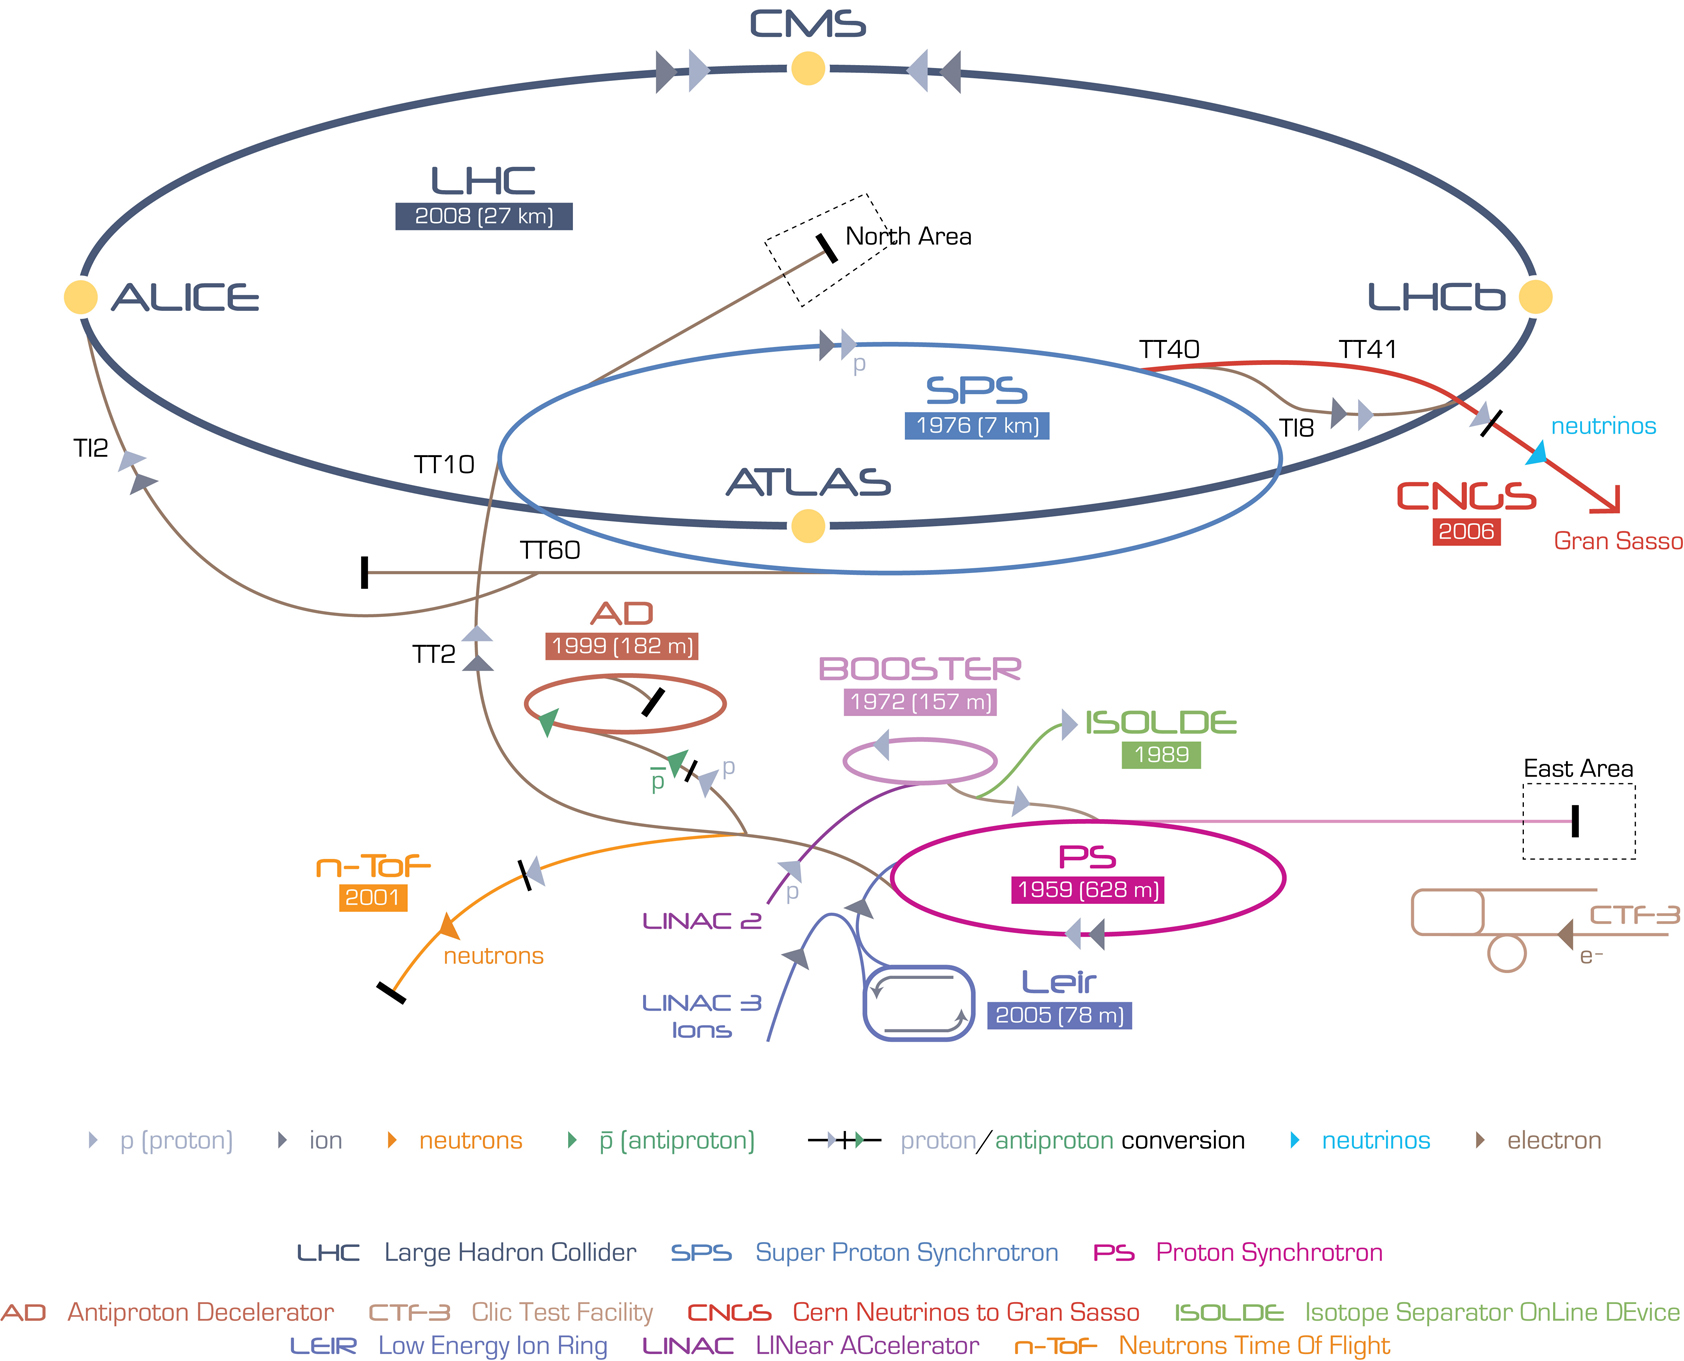
\includegraphics[width=0.8\textwidth]{figures/exp/accelerators.jpg}
\caption{The LHC accelerator complex}
\label{fig:lhc_accelerators}
\end{centering}
\end{figure}

The proton-proton collisions at the LHC interaction points result in a number of events per second given by~$N_i = L \sigma_i$~for a process that has a cross-section~$\sigma_i$~at a given instantaneous luminosity~$L$. For the LHC, the machine luminosity is given by the Gaussian beam profile through

\begin{equation}
L = \frac{N_b^2 n_b f_\mathrm{rev} \gamma_r}{4 \pi \epsilon_n \beta^*} F.
\end{equation}
where~$f_{\mathrm{rev}}$~is the number of revolutions per second and~$\gamma_r$~is the relativistic Lorentz factor. The beam is further described by the normalized transverse emittance~$\epsilon_n$~and the beta function~$\beta^*$~of the beam at the interaction point, which are related to the transverse beam size at a location~$s$~along the beam through~$\sigma(s) = \sqrt{\epsilon_n \beta(s)}$. The transverse emittance characterizes the spread of particles position-momentum phase throughout their orbits. The beams cross at an angle~$\theta_c$, which results in the luminosity reduction factor

\begin{equation}
F = \biggl[1 + \bigr( \frac{\theta_c \sigma_z}{2 \sigma^*} \bigr)^2 \biggr]^{-1/2}
\end{equation}
where~$\sigma_z$~is the bunch length and~$\sigma^*$~the transverse bunch size. The~$\beta^*$~parameter dictates the size of the beam at the interaction point, which is tuned to the luminosity requirements of the experiment and in turn limited by the aperture of the focusing magnets. The maximum beam size in the transverse direction is~$\sigma=1.2~\mathrm{mm}$, limited by the dimensions of the beam screen. The instantaneous luminosity decays over time during a physics run due to beam loss from the collisions, such that the luminosity decreases by~$1/e$~during approximately~$15\ h$.

The total number of collisions in a given unit of time is characterized by the integrated luminosity~$\mathcal{L} = \int L\ \mathrm{d}t$~and is limited to around~$80-120~\mathrm{fb}^{-1}$~per year, assuming around 200 days of operation and on average 7 hours of turn-around time between runs for filling the beams and accelerating to data-taking energies.

During the 2016 data taking period considered in this thesis, the LHC operated at a center-of-mass energy of~$\sqrt{s} = 13~\mathrm{TeV}$,~$\beta^* = 40~\mathrm{cm}$~and delivered around~$\mathcal{L} = 40~\mathrm{fb}^{-1}$~of proton-proton data to the ATLAS and CMS experiments. With an inelastic pp cross-section of~$\sigma_{pp} \simeq 77$~mb~\cite{VanHaevermaet:2016gnh}, this correspond to about~$10^{15}$~pp interactions.

The collision data form the LHC is recorded by 2 general purpose detectors, CMS and ATLAS (A Toroidal LHC ApparatuS), and 2 experiments with a more specialized physics program, LHCb and ALICE (A Large Ion Collider Experiment), located at the interaction points:

\begin{itemize}
    \item \textbf{CMS}: The main characteristic of CMS is the superconducting solenoid, which provides a magnetic field of 3.8T that enables the momentum of charged particles to be measured with high accuracy. Inside the solenoid volume are silicon pixel and strip trackers, an electromagentic calorimeter (ECAL) comprised of~$\mathrm{PbWO}_4$~crystals and a brass-scintillator hadronic calorimeter (HCAL). Outside the solenoid volume is the steel return yoke for the magnetic field, which contains gas-ionization chambers used to measure muons. The CMS detector was designed to meet a dimuon, diphoton and dielectron mass resolution of~$1\%$~at 100~GeV~\cite{Chatrchyan:2008aa}.
    \item \textbf{ATLAS}: The overall layout of the ATLAS machine differs from CMS mainly with respect to the configuration of the magnetic fields, where a central superconducting solenoid with B=2T houses the semiconductor trackers, with the lead-liquid argon (LAr) electromagnetic calorimeter and the hadronic calorimeters outside the solenoid volume. The muon systems are embedded in an outer air-core toroidal system that minimizes multiple scattering. The CMS
    \item \textbf{LHCb}: The primary goal of the LHCb experiment is dedicated to heavy flavour physics, in particular rare decays of beauty and charm hadrons and indirect evidence for new physics in CP-violation, exploiting the large rate of B-meson production at the LHC. The LHCb detector is a single-arm spectrometer with a forward angular coverage of 10 to 250-300~mrad, featuring a beryllium beampipe that is highly transparent to particle fluxes. LHCb operates at an instantaneous luminosity that is two orders of magnitude lower than CMS and ATLAS in order to minimize multiple pp interactions per bunch crossing.
    \item \textbf{ALICE}: The ALICE detector is designed to study heavy ions, focusing on QCD measurements, in particular to study the nature of strongly interacting matter at the high temperatures and densities achievable in nucleon-nucleon collisions. It features a general-purpose detectors in the barrel, embedded in a solenoid and muon spectrometers in the forward direction. The ALICE detector is specifically optimized to study global event observables such as particle multiplicity and energy flow. 
\end{itemize}
In the following section, we will discuss the essential aspects of the CMS experiment in more detail.

\subsection{The CMS detector}
The coordinate system adopted by CMS is centered at the collision point, with the x-axis pointing inward towards the LHC ring, y-axis vertically upward and the z axis along the beamline towards east in the direction of the Jura mountains. The azimuthal angle~$\phi$~is measured from the x axis in the plane transverse to the beam. The polar angle is measured from the z-axis and it defines the pseudorapidity~$\eta = -\ln{\tan{\theta/2}}$. The CMS detector follows a layered design that encapsulates the interaction region completely in the azimuthal direction and provides good coverage in the polar direction. In order to achieve this, the detector is divided into a barrel component and two endcaps, as can be seen on~\cref{fig:cms_experiment}.

\begin{figure}
\begin{centering}
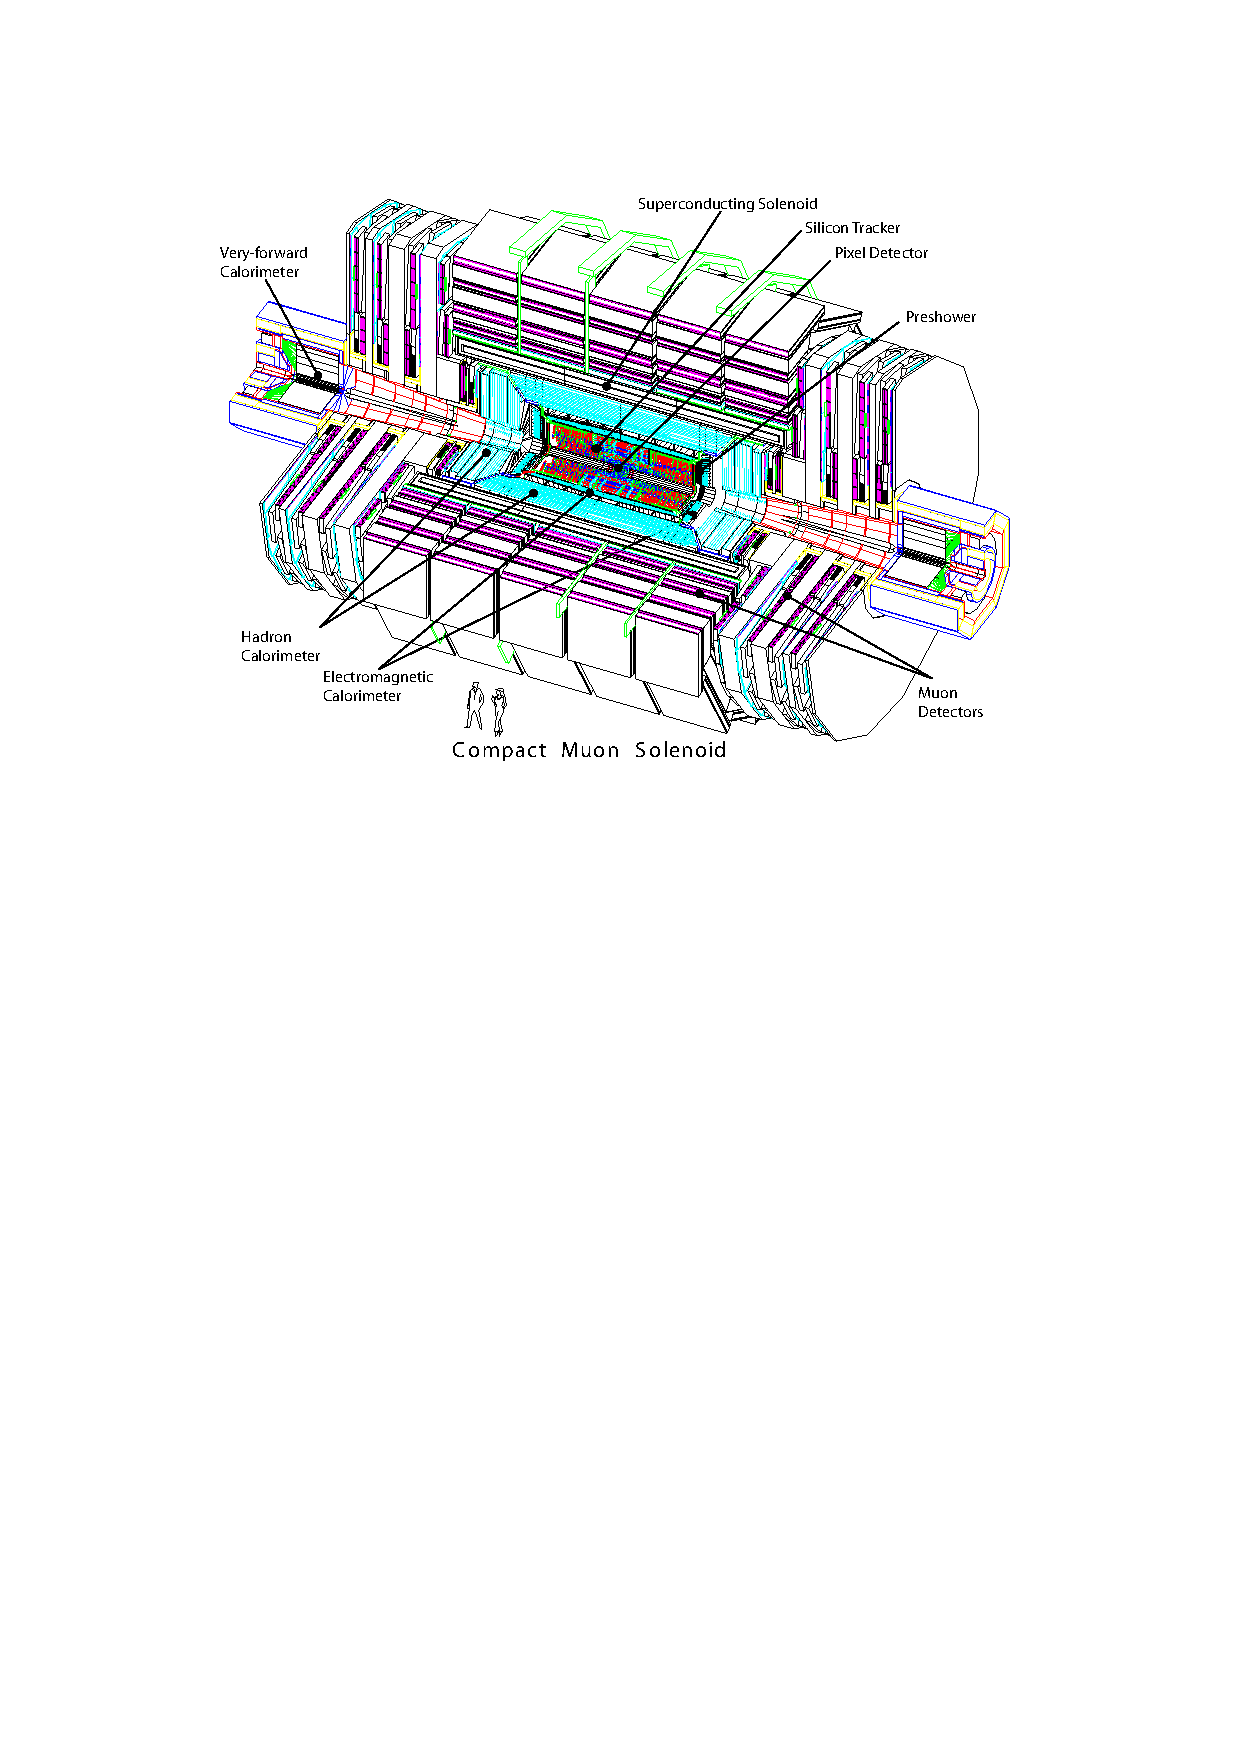
\includegraphics[width=0.8\textwidth]{figures/exp/cms.pdf}
\caption{The cross-section of the CMS experiment.}
\label{fig:cms_experiment}
\end{centering}
\end{figure}


\subsubsection{The superconducting magnet}

The 3.8T magnetic field, which is essential for measuring the momenta and charge of charged particles, is created by the 220~ton superconducting solenoid, which has a diameter of 6~m and a length of 12.5~m. The energy stored in the NbTi conductor reaches up to 2.6~GJ, therefore the mechanical deformations in the magnet during energizing can be significant. The return yoke of the magnetic field consists of sections which house the muon chambers and thus guarantees a sufficient field strength in the muon spectrometer region.

\subsubsection{Inner tracking system}
The inner tracking system measures the momenta and trajectories of charged particles from the primary vertex in the interaction point and any secondary vertices associated to the decay of long-lived particles. The magnetic field is homogeneous within the tracker volume, which has a length of 5.8~m and a diameter of 2.5~m. The number of simultaneous inelastic collision (pileup) events per bunch crossing in pp collisions can be significant at the LHC, with nominal values around~$N_{PV} = 20$, but reaching an order of magnitude more in the HL-LHC. Therefore, the tracking system has to cope with high particle fluxes of up to~$10^3$~particles per bunch crossing every 25~ns and be able to associate signals to the correct bunch crossing. In order to keep the hit occupancy around 1\%, pixel detectors have to be used in the inner region of the tracker. The inner tracker consists of a 3-layer silicon pixel detector with layers at 4.4~cm, 7.3~cm and 10.2~cm and a silicon strip detector with 10 layers extending out to radii of 1.1~m. The pixels in the inner layer measure~$100\times150~\mathrm{\mu m}^2$~in the~$r-\phi$~and~$z$~directions, which is driven by the secondary vertex and impact parameter resolution necessary for the detection of heavy flavour states. The pixel detector covers the range range~$|\eta| < 2.5$~and consists of the barrel layers (BPix) and two endcap discs (FPix), located in such a way as to guarantee at least 3 pixel hits over almost the full range, as seen on~\cref{fig:cms_pixel}. By reading out the analog pulse height using charge sharing which results from the the B field, a hit resolution of 15-20~$\mathrm{\mu m}$~can be achieved. In total, the pixel detector covers an area of~$1~\mathrm{m}^2$~and consists of around 66 million pixels.

\begin{figure}
\begin{centering}
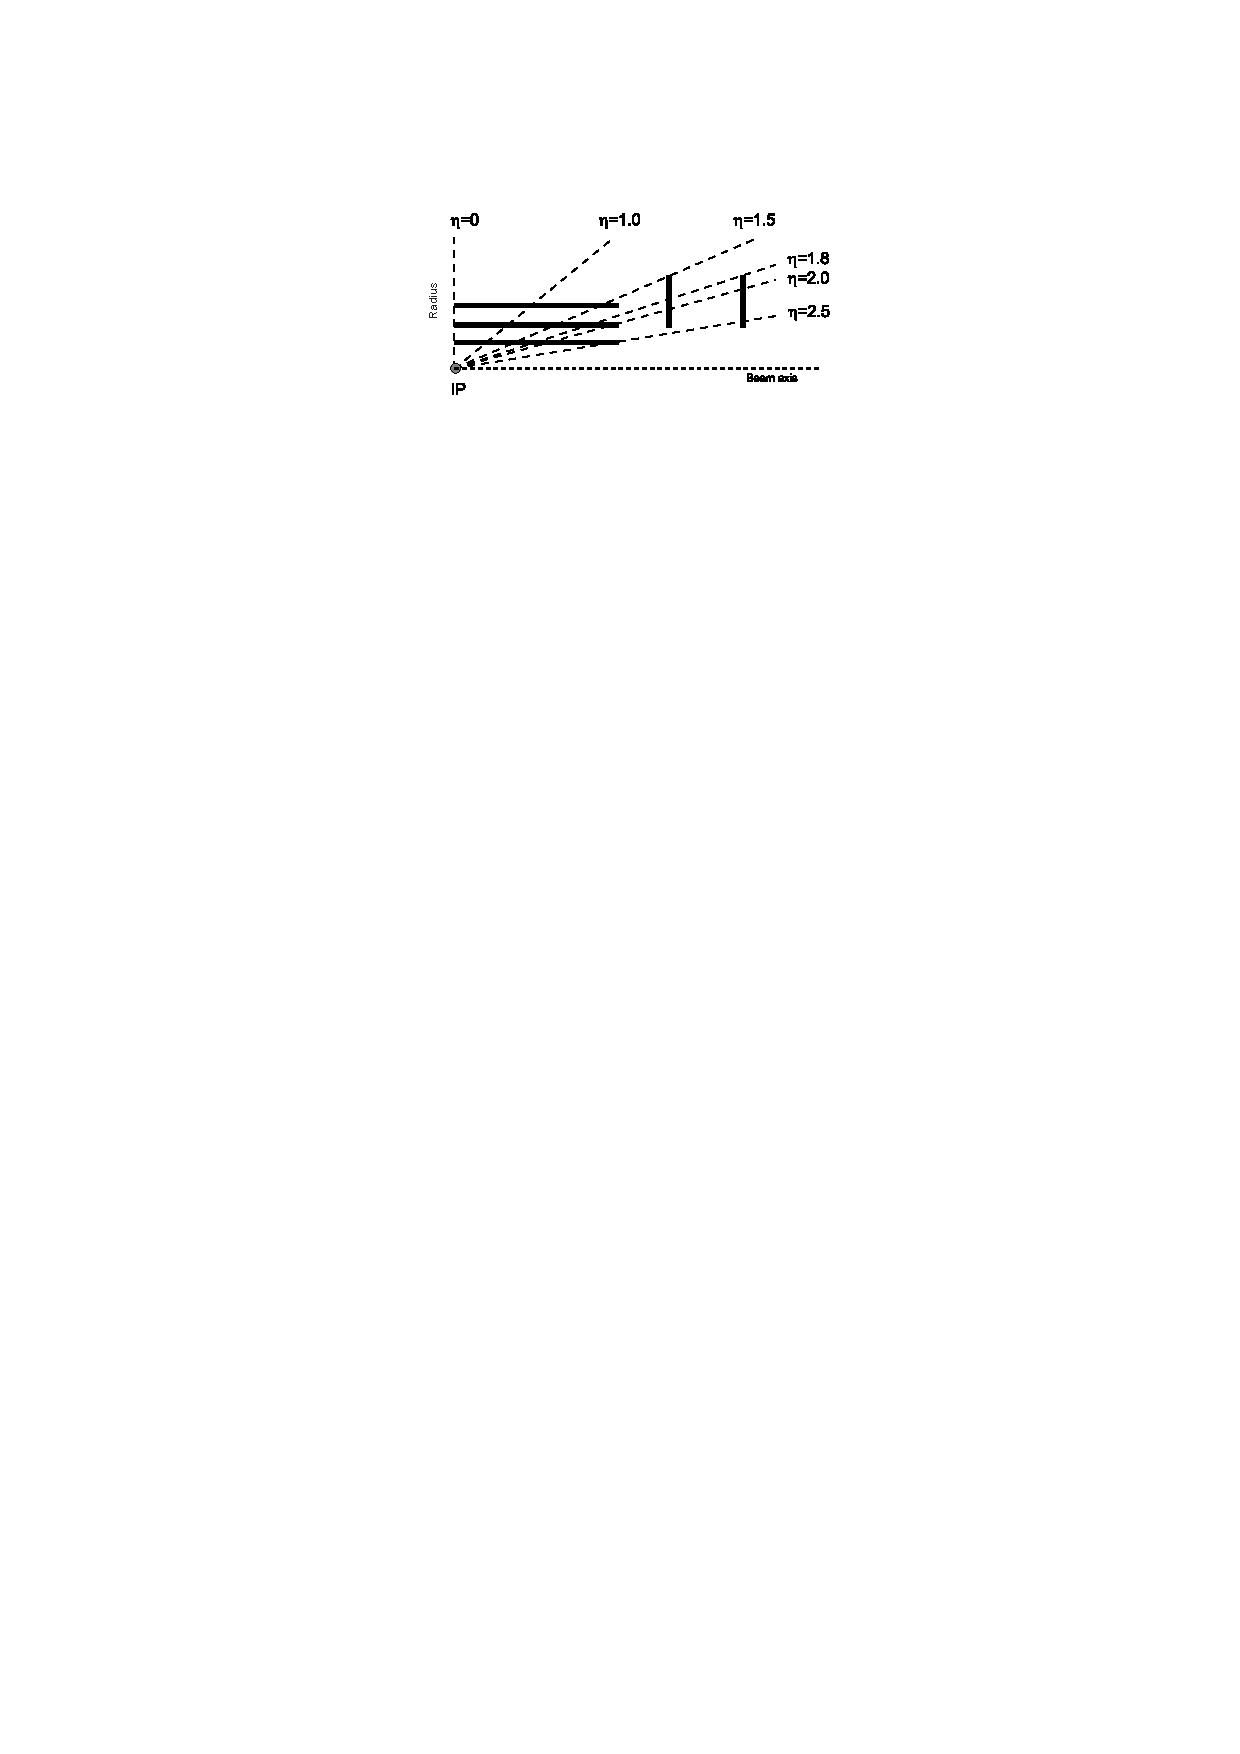
\includegraphics[width=0.6\textwidth]{figures/exp/pixel.pdf}
\caption{The schematic overview of the CMS pixel tracker.}
\label{fig:cms_pixel}
\end{centering}
\end{figure}

At larger radii, the occupancy decreases, such that silicon strips with a typical size of~$10\mathrm{cm} \times 80\mathrm{\mu m}$~are used in the silicon strip tracker. The tracker consists of several layered subsystems as shown on~\cref{fig:cms_tracker}, in particular, the tracker inner barrel and discs (TIB/TID), the outer barrel (TOB) and the tracker endcaps (TEC). The TIB/TID delivers 4 measurements of a track in the~$r-\phi$~direction, the TOB 6 measurements, and the TEC 9 measurements per particle trajectory. The strip pitch increases at larger radii to compensate for the reduction in particle flux.

\begin{figure}
\begin{centering}
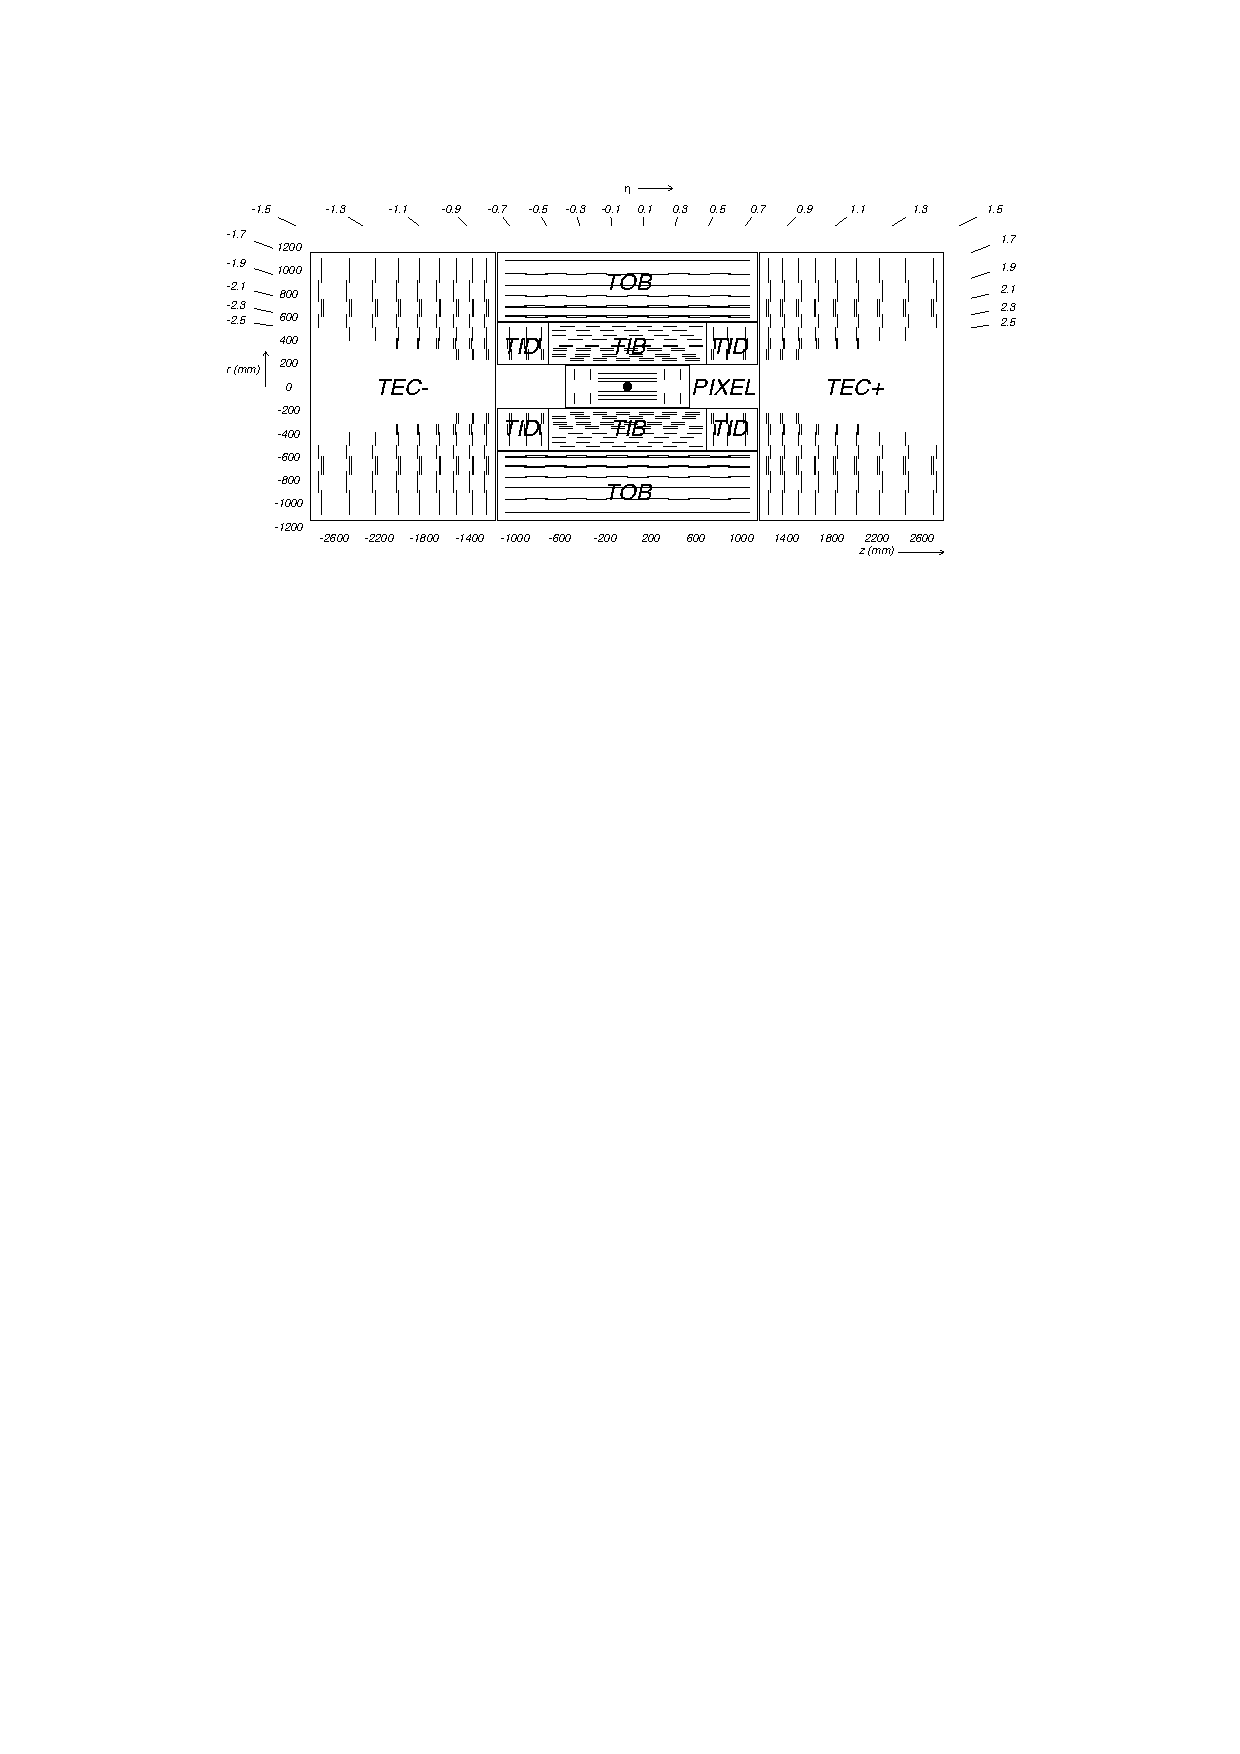
\includegraphics[width=0.6\textwidth]{figures/exp/tracker.pdf}
\caption{The schematic overview of the CMS strip tracking system.}
\label{fig:cms_tracker}
\end{centering}
\end{figure}

Overall, the tracking system has to maximize the number of measurements for each trajectory while keeping the material budget, measured in radiation lengths~$X_0$, at a minimum. Over the whole functional~$\eta$~range, the tracking system contributes between 0.4 and 1.8~$X_0$, with the largest radiation losses in the region around~$|\eta| \simeq 1.5$~due to the TIB/TID transition. Nevertheless, the transverse momentum resolution of muons is around~$1-2\%$~up to~$|\eta| \leq 1.6$, a reconstruction efficiency of around 99\% over most of the~$\eta$~range and of the transverse impact parameter resolution around~$10~\mathrm{\mu m}$~for high momentum tracks. 

The pixel detector was upgraded during the 2016-2017 winter shutdown procedure, adding an additional layer at~$r=2.9$~cm and improving the capabilities of the readout chip (ROC) to cope with an instantaneous luminosity of~$L = 2 \times 10^{34}\ \mathrm{cm}^{-2}\mathrm{s}^{-1}$~\cite{Tavolaro:2016hfj}.

\subsubsection{Electromagnetic calorimeter}
The primary function of the electromagnetic calorimeter is to measure the energy of electrons and photons through the production of scintillation light with sufficient resolution to reconstruct the decay of the Higgs boson to 2 photons. The ECAL is situated within the solenoid volume in order to minimize energy losses from multiple scattering and consists of around 76000 lead-tungstenate~($\mathrm{PbWO}_4$) crystals arranged in the barrel and endcap, as seen on~\cref{fig:cms_ecal}. This material is characterized by a high density~($\rho = 8.28~\mathrm{g}/\mathrm{cm}^3$), a short radiation length ($X=0.89~\mathrm{cm}$) and a small Moliere radius~(2.19~cm). Furthermore, the scintillation decay time is short, such that 80\% of the light is emitted during the 25~ns bunch spacing. In the barrel (endcaps), the crystals are coupled to avalanche photodiodes (vacuum phototriodes) for light collection. Due to the high radiation damage expected throughout the lifetime of the ECAL, the light transmission properties of the crystals are monitored using injected laser light at $\lambda = 440~\mathrm{nm}$. A two-layer lead absorber and silicon strip sensor preshower detector is located between the endcaps and the interaction point, covering $1.65 < |\eta| < 2.6$, in order to improve the discrimination between photons and $\pi^0$.

\begin{figure}
\begin{centering}
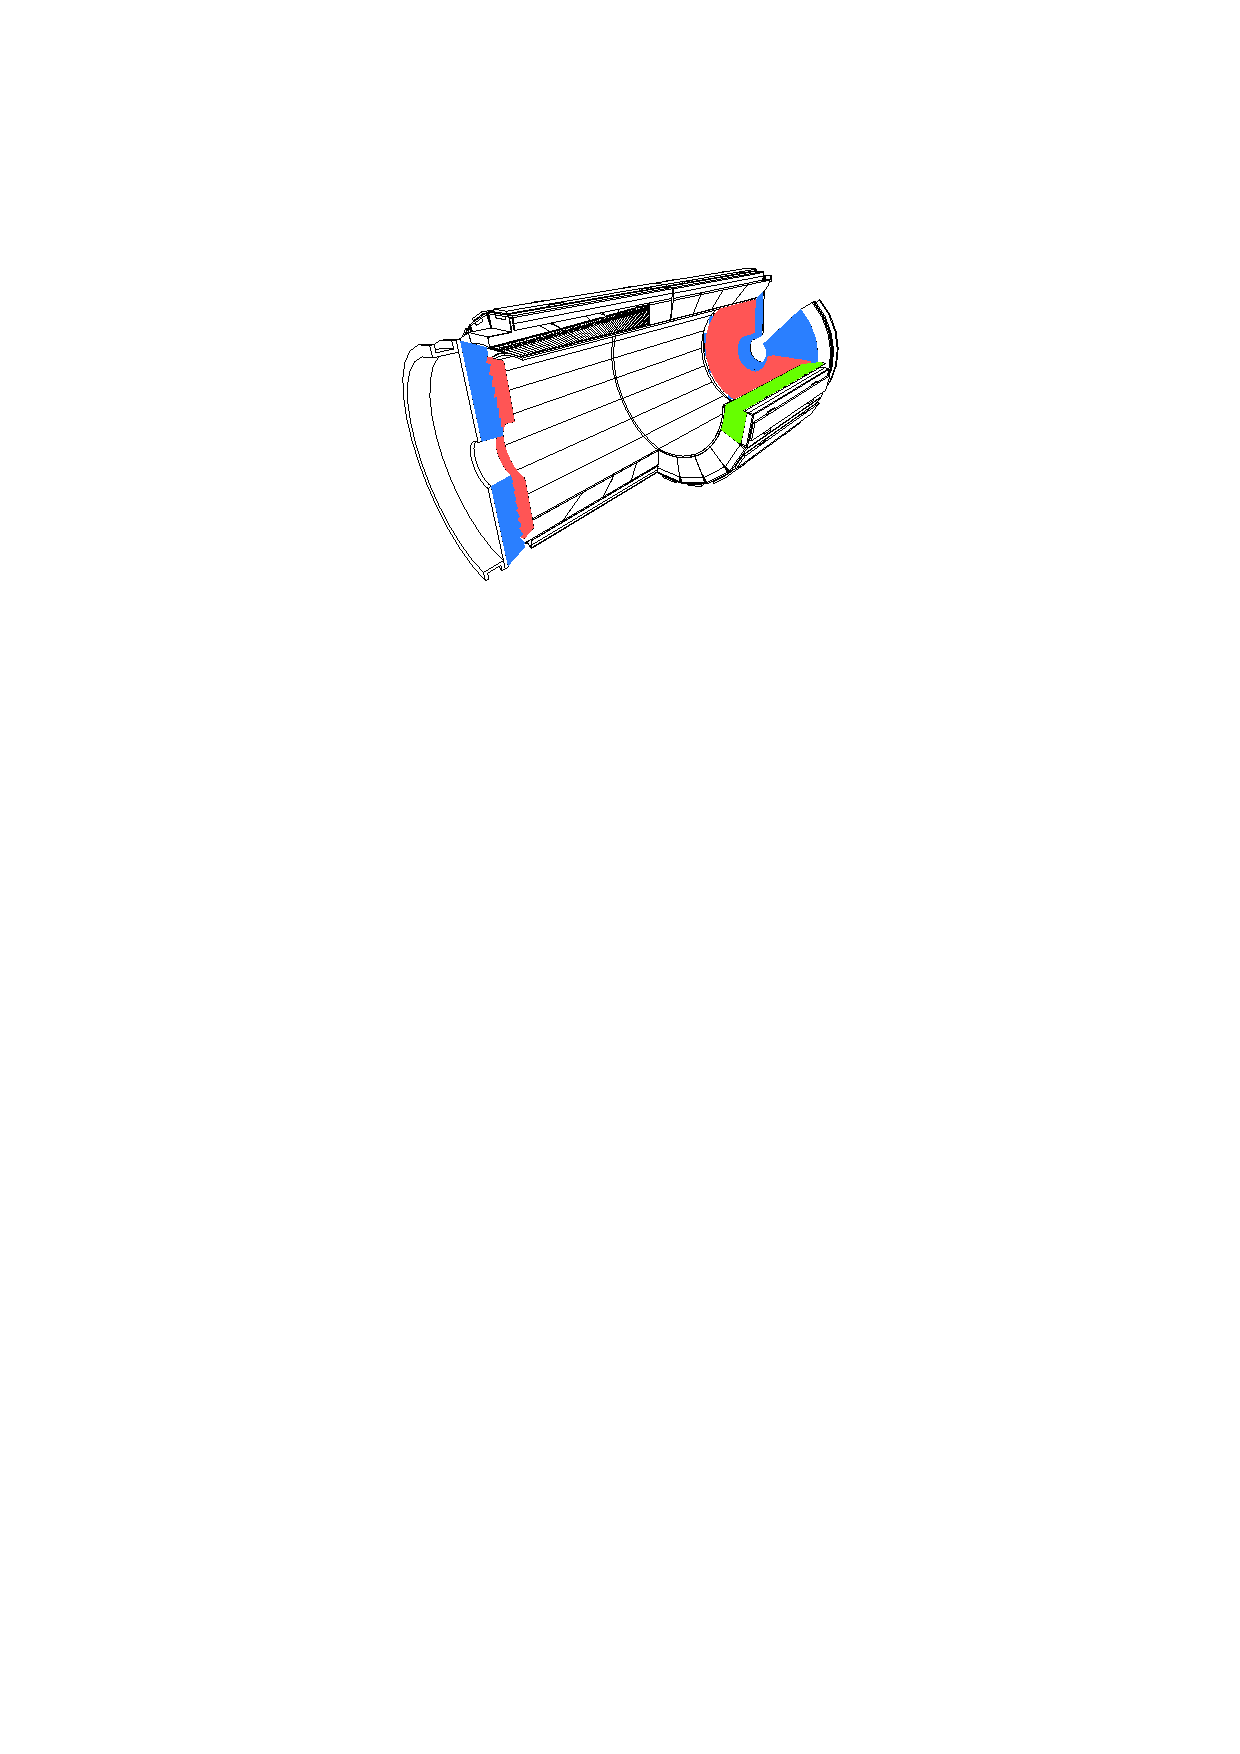
\includegraphics[width=0.6\textwidth]{figures/exp/ecal.pdf}
\caption{The CMS electromagnetic calorimeter.}
\label{fig:cms_ecal}
\end{centering}
\end{figure}

The ECAL barrel region extends to~$|\eta| < 1.479$, with a 360-fold (190-fold) granularity in the azimuthal (polar) direction and the endcaps between~$1.479 < |\eta| < 3.0$. The endcaps are grouped to $5\times5$ superclusters of crystals. Since the photon emission in scintillation and subsequent amplification are temperature-dependent, the ECAL has to be maintained at a constant temperature of~$18\deg \mathrm{C}$.

In order to reconstruct the signal pulse from the photodetectors, a new technique is used in Run II, where the signal amplitude templates from up to 9 bunch crossings around the in-time signal are fitted to the observed 10-sample signal, in order to determine signal amplitude~\cite{Brianza:2017slq}.

The energy resolution of the ECAL has been measured in electron test beams, arranging the crystals in either a $3\times3$ or $5\times5$ matrix, and found to be

\begin{equation}
\frac{\sigma_E}{E} = \frac{a}{\sqrt{E}} \oplus \frac{b}{E} \oplus c
\end{equation}
with $a = 2.8\%$ being the stochastic term, $b = 12\%$ the noise term and $c = 0.3\%$ the irreducible term from non-uniformities for the barrel~\cite{Adzic:2007mi}.